% vim: set tw=80:spell
%
\documentclass[twoside,a5paper,10pt]{extarticle}
%\documentclass[twoside,14pt,draft]{extarticle}
%\documentclass[twoside,14pt,draft]{scrartcl}
\usepackage{amsmath}
\usepackage{amssymb}
\usepackage{amsfonts}
\usepackage{mathtext}
\usepackage{pdfpages}
\usepackage{parallel}
\usepackage[T2A]{fontenc}
\usepackage{ucs}
\usepackage[utf8x]{inputenc}
\usepackage[polish,english,russian]{babel}
\usepackage{hyperref}
\usepackage{rotating}
\usepackage[inner=2cm,top=1.8cm,outer=2cm,bottom=2.3cm,nohead]{geometry}
\usepackage{listings}
\usepackage{graphicx}
\usepackage{wrapfig}
\usepackage{longtable}
\usepackage{indentfirst}
\usepackage{array}
\newcolumntype{P}[1]{>{\raggedright\arraybackslash}p{#1}}
\frenchspacing
\usepackage{fixltx2e} %text sub- and superscripts
\usepackage{icomma} % коскі ў матэматычным рэжыме
\PreloadUnicodePage{4}

\newcommand{\longpage}{\enlargethispage{\baselineskip}}
\newcommand{\shortpage}{\enlargethispage{-\baselineskip}}

\def\switchlang#1{\expandafter\csname switchlang#1\endcsname}
\def\switchlangbe{
\let\saverefname=\refname%
\def\refname{Літаратура}%
\def\figurename{Іл.}%
}
\def\switchlangen{
\let\saverefname=\refname%
\def\refname{References}%
\def\figurename{Fig.}%
}
\def\switchlangru{
\let\saverefname=\refname%
\let\savefigurename=\figurename%
\def\refname{Литература}%
\def\figurename{Рис.}%
}

\hyphenation{admi-ni-stra-tive}
\hyphenation{ex-pe-ri-ence}
\hyphenation{fle-xi-bi-li-ty}
\hyphenation{Py-thon}
\hyphenation{ma-the-ma-ti-cal}
\hyphenation{re-ported}
\hyphenation{imp-le-menta-tions}
\hyphenation{pro-vides}
\hyphenation{en-gi-neering}
\hyphenation{com-pa-ti-bi-li-ty}
\hyphenation{im-pos-sible}
\hyphenation{desk-top}
\hyphenation{elec-tro-nic}
\hyphenation{com-pa-ny}
\hyphenation{de-ve-lop-ment}
\hyphenation{de-ve-loping}
\hyphenation{de-ve-lop}
\hyphenation{da-ta-ba-se}
\hyphenation{plat-forms}
\hyphenation{or-ga-ni-za-tion}
\hyphenation{pro-gramming}
\hyphenation{in-stru-ments}
\hyphenation{Li-nux}
\hyphenation{sour-ce}
\hyphenation{en-vi-ron-ment}
\hyphenation{Te-le-pathy}
\hyphenation{Li-nux-ov-ka}
\hyphenation{Open-BSD}
\hyphenation{Free-BSD}
\hyphenation{men-ti-on-ed}
\hyphenation{app-li-ca-tion}

\def\progref!#1!{\texttt{#1}}
\renewcommand{\arraystretch}{2} %Іначай формулы ў матрыцы зліпаюцца з лініямі
\usepackage{array}

\def\interview #1 (#2), #3, #4, #5\par{

\section[#1, #3, #4]{#1 -- #3, #4}
\def\qname{LVEE}
\def\aname{#1}
\def\q ##1\par{{\noindent \bf \qname: ##1 }\par}
\def\a{{\noindent \bf \aname: } \def\qname{L}\def\aname{#2}}
}

\def\interview* #1 (#2), #3, #4, #5\par{

\section*{#1\\{\small\rm #3, #4. #5}}

\def\qname{LVEE}
\def\aname{#1}
\def\q ##1\par{{\noindent \bf \qname: ##1 }\par}
\def\a{{\noindent \bf \aname: } \def\qname{L}\def\aname{#2}}
}

%\usepackage{portland}
%\usepackage{lscape}
%\usepackage{rotating}
\usepackage[labelsep=period,justification=centering]{caption}
%\usepackage{ccaption}
%\captiondelim{. }
\usepackage{tweaklist}
%\usepackage{trace}
%\usepackage{tikz}
%\usetikzlibrary{calc}
%\usetikzlibrary{positioning}
\usepackage{subfig}
\renewcommand{\enumhook}{\setlength{\topsep}{0pt}%
  \setlength{\itemsep}{0pt}\setlength{\parskip}{0pt plus 1pt minus 1pt}\setlength{\parsep}{0pt}}
\renewcommand{\itemhook}{\setlength{\topsep}{0pt}%
  \setlength{\itemsep}{0pt}\setlength{\parskip}{0pt plus 1pt minus 1pt}\setlength{\parsep}{0pt}}
%\renewcommand{\enumhook}{\setlength{\topsep}{0pt}%
%  \setlength{\itemsep}{0pt}}
%\renewcommand{\itemhook}{\setlength{\topsep}{0pt}%
%  \setlength{\itemsep}{0pt}\setlength{\parskip}{0pt}\setlength{\parsep}{0pt}}
%\renewcommand{\enumhook}{\setlength{\topsep}{0pt}%
%  \setlength{\itemsep}{0pt}}
%\renewcommand{\itemhook}{\setlength{\topsep}{0pt}%
%  \setlength{\itemsep}{0pt}\setlength{\parsep}{0pt}}

\clubpenalty=10000%
\widowpenalty=10000%
%\setlength{\parindent}{1.25cm}%

\newcommand\familyname[1]{\textbf{#1}}

\DeclareMathOperator{\e}{e}
\DeclareMathOperator{\cov}{cov}
\DeclareMathOperator{\diag}{diag}

\newcommand{\longpage}{\enlargethispage{\baselineskip}}
\newcommand{\shortpage}{\enlargethispage{-\baselineskip}}

\newcommand\eof{\writetotalpages\end{document}\endinput}

\newcommand\key[1]{\textbf{#1}}
\newcommand\vect[1]{\mathbf{#1}}
\def\eqn #1 $#2${\begin{equation}\label{eq:#1}#2\end{equation}}
%\def\where #1
\newcommand\eqnref[1]{(\ref{eq:#1})}
\makeatletter
\def\p@subfigure{\thefigure,~}
\def\thesubfigure{\asbuk{subfigure}}
\@newctr{figure}
\renewcommand \thefigure {\@arabic\c@figure}
\@newctr{equation}
\renewcommand\theequation{\@arabic\c@equation}
\newcommand\ps@twoside{%
 \makeatletter%
 \renewcommand\@oddfoot{~\hfill\thepage}%
 \renewcommand\@evenfoot{\thepage\hfill~}%
 \makeatother%
}
\newcounter{totalpages}
\def\writetotalpages{%
  \protected@write\@auxout
      {}%
      {\string\setcounter{totalpages}{\thepage}}}
\newcounter{totalfigures}%
\newcounter{totalsubfigures}%
\newcounter{totalsections}%
\newcounter{totalsubsections}%
\newcounter{totalsubsubsections}%
\newcounter{totalparagraphs}%

\def\addcontentsline#1#2#3{%
  \addtocontents{#1}{\protect\contentsline{#2}{#3}{\thepage}%
  \protect\stepcounter{total#2s}}}
\makeatother
\newcommand\comment[1]{\textsf{#1}}
\renewcommand\labelitemi{\textendash}
\renewcommand\labelitemii{\textendash}


% перенос формул в тексте
\newcommand*{\hm}[1]{#1\nobreak\discretionary{}%
  {\hbox{$\mathsurround=0pt #1$}}{}}

\def\layersep{2.5cm}

\begin{document}
\pagestyle{twoside}

\thispagestyle{empty}
\newpage
\tableofcontents

\def\documentclass[#1]#2{}

\makeatletter

\def\@self@name{00}
\def\@preamble@name{preamble.tex}

\def\document{\newpage}
\let\@lvee@enddoc\enddocument

\let\@lvee@input\input
\def\enddocument{%
\gdef\@title{}%
\gdef\@author{}%
}

\renewcommand\maketitle{\par
  \begingroup
    \renewcommand\thefootnote{\@fnsymbol\c@footnote}%
    \def\@makefnmark{\rlap{\@textsuperscript{\normalfont\@thefnmark}}}%
    \long\def\@makefntext##1{\parindent 1em\noindent
            \hb@xt@1.8em{%
                \hss\@textsuperscript{\normalfont\@thefnmark}}##1}%
    \if@twocolumn
      \ifnum \col@number=\@ne
        \@maketitle
      \else
        \twocolumn[\@maketitle]%
      \fi
    \else
      \newpage
      \global\@topnum\z@   % Prevents figures from going at top of page.
      \@maketitle
    \fi
    \thispagestyle{plain}\@thanks
  \endgroup
}

\def\input#1{
\def\@@@curfile{#1}
\message{@@\@@@curfile @@}
\ifx \@@@curfile \@preamble@name
    \message{An attempt to include the preamble has occured, ignoring.^^J}
\else
    \ifx \@@@curfile \@self@name
        \message{An attempt to include ourselves had occured, ignoring.^^J}
    \else
        \@lvee@input#1
    \fi
\fi
}
\makeatother

\documentclass[10pt, a5paper]{article}
\usepackage{pdfpages}
\usepackage{parallel}
\usepackage[T2A]{fontenc}
\usepackage{ucs}
\usepackage[utf8x]{inputenc}
\usepackage[polish,english,russian]{babel}
\usepackage{hyperref}
\usepackage{rotating}
\usepackage[inner=2cm,top=1.8cm,outer=2cm,bottom=2.3cm,nohead]{geometry}
\usepackage{listings}
\usepackage{graphicx}
\usepackage{wrapfig}
\usepackage{longtable}
\usepackage{indentfirst}
\usepackage{array}
\newcolumntype{P}[1]{>{\raggedright\arraybackslash}p{#1}}
\frenchspacing
\usepackage{fixltx2e} %text sub- and superscripts
\usepackage{icomma} % коскі ў матэматычным рэжыме
\PreloadUnicodePage{4}

\newcommand{\longpage}{\enlargethispage{\baselineskip}}
\newcommand{\shortpage}{\enlargethispage{-\baselineskip}}

\def\switchlang#1{\expandafter\csname switchlang#1\endcsname}
\def\switchlangbe{
\let\saverefname=\refname%
\def\refname{Літаратура}%
\def\figurename{Іл.}%
}
\def\switchlangen{
\let\saverefname=\refname%
\def\refname{References}%
\def\figurename{Fig.}%
}
\def\switchlangru{
\let\saverefname=\refname%
\let\savefigurename=\figurename%
\def\refname{Литература}%
\def\figurename{Рис.}%
}

\hyphenation{admi-ni-stra-tive}
\hyphenation{ex-pe-ri-ence}
\hyphenation{fle-xi-bi-li-ty}
\hyphenation{Py-thon}
\hyphenation{ma-the-ma-ti-cal}
\hyphenation{re-ported}
\hyphenation{imp-le-menta-tions}
\hyphenation{pro-vides}
\hyphenation{en-gi-neering}
\hyphenation{com-pa-ti-bi-li-ty}
\hyphenation{im-pos-sible}
\hyphenation{desk-top}
\hyphenation{elec-tro-nic}
\hyphenation{com-pa-ny}
\hyphenation{de-ve-lop-ment}
\hyphenation{de-ve-loping}
\hyphenation{de-ve-lop}
\hyphenation{da-ta-ba-se}
\hyphenation{plat-forms}
\hyphenation{or-ga-ni-za-tion}
\hyphenation{pro-gramming}
\hyphenation{in-stru-ments}
\hyphenation{Li-nux}
\hyphenation{sour-ce}
\hyphenation{en-vi-ron-ment}
\hyphenation{Te-le-pathy}
\hyphenation{Li-nux-ov-ka}
\hyphenation{Open-BSD}
\hyphenation{Free-BSD}
\hyphenation{men-ti-on-ed}
\hyphenation{app-li-ca-tion}

\def\progref!#1!{\texttt{#1}}
\renewcommand{\arraystretch}{2} %Іначай формулы ў матрыцы зліпаюцца з лініямі
\usepackage{array}

\def\interview #1 (#2), #3, #4, #5\par{

\section[#1, #3, #4]{#1 -- #3, #4}
\def\qname{LVEE}
\def\aname{#1}
\def\q ##1\par{{\noindent \bf \qname: ##1 }\par}
\def\a{{\noindent \bf \aname: } \def\qname{L}\def\aname{#2}}
}

\def\interview* #1 (#2), #3, #4, #5\par{

\section*{#1\\{\small\rm #3, #4. #5}}

\def\qname{LVEE}
\def\aname{#1}
\def\q ##1\par{{\noindent \bf \qname: ##1 }\par}
\def\a{{\noindent \bf \aname: } \def\qname{L}\def\aname{#2}}
}


\begin{document}

\title{Cells.js --- еще один подход к разработке современных веб-приложений}

\author{Алексей Кондратенко\\
\small Altoros Development, \texttt{alk@tut.by}
}
\maketitle

\begin{abstract}
Membase NoSQL database management system has administrative interface 
implemented as modern ``single-page'' aka ``pure-js'' web application. 
This talk will describe Cells.js --- a library that was grown inside 
this user interface component. It facilitates structuring of user 
interface as a collection of inter-dependent variables or cells. This 
provides some otherwise hard to implement features, like back button 
support, for free. And I believe, that this leads to cleaner and smaller 
code base.
\end{abstract}

В последние годы получила распостранение такая практика организации
веб-приложений, когда на стороне браузера реализуется вся логика
пользователького интерфейса. Серверная сторона при этом предоставляет
только <<голый>> API для доступа к данным. Преимуществом такого подхода
является более отзывчивый интерфейс, т.к. реакция на действия
пользователя реализуется на стороне браузера.

Одной из проблем построения пользователького интерфейса в таком виде
является относительная неадаптированность современных web-стандартов
к такого рода приложениям. Эти стандарты создавались в основном для
статического web. Другой известной проблемой является неполная или
неправильная реализация стандартов в разных браузерах.

Для реализации несложной логики зачастую достаточно применить одну из
библиотек для кросс-браузерного манипулирования DOM и кросс-браузерной
реализации \verb!XMLHttpRequest!. В последнее время в этой нише доминирует
библиотека jquery. Реализация более сложной логики быстро превращает
код в запутанную и трудно поддерживаемую кашу из обработчиков событий и 
требует перехода к какому-либо способу организации более богатого
пользователького интерфейса.

К одному из таких способов относятся MVC и его производные. На
сегодняшний день имеется масса тяжеловесных фреймворков для
реализации MVC, например Google Web Toolkit, ExtJS, SproutCore.

Однако, на мой взгляд, в средних по размеру приложениях применение более
компактных и простых решений оправдано.

При создании web-интерфейса для Membase было изначально решено
использовать только jquery. Однако после реализации первых экранов я
понял, что без более продвинутой организации логики этот код будет
невозможно поддерживать и развивать.

Большинство MVC-фреймворков имеет в своем основании систему наблюдения
за данными и реакции на их изменения. Это позволяет отделять логику
получения/обработки данных от логики обработки пользователькой реакции
и логики представления этих данных пользователю.

Я начал с создания простого класса, реализующего наблюдаемое значение и
возможность <<подписаться>> на его измeнения. Это помогло
структурировать код лучше. Но затем я заметил, что некоторые значения
полностью детерминированно зависят от других значений. Я вспомнил про
проект cells, реализованный на common-lisp 
(\url{http://common-lisp.net/project/cells/}) и понял, что могу легко
реализовать основную идею этого проекта на javascript.

В результате пользователький интерфейс Membase (и до этого Northscale
Memcached Server) организован как набор связаных зависимостями по
данным ячеек. Большинство ячеек является вычисляемыми, т.е. каждой из
них соответствует детерминированная функция на javascript. Значения
функций вычисляемых ячеек могут зависеть только от значений других
ячеек. И библиотека организует (пере)вычисления ячеек когда значения
их зависимостей либо становится известно, либо изменяется.

Когда одной из исходных ячеек присваивается какое-либо значение,
например, в результате действия пользователя, cells.js организует
перевычисление всех ячеек, которые зависят от этой ячейки. После чего
перевычисляются ячейки, зависимые от только что перевычисленных ячеек, и
так далее. T.e. cells.js организует <<расплывание>> данных (и, в
некотором роде, реакции) по ячейкам.

Видимые пользователью блоки пользователького интерфейса подписываются
на значениe ячейки, которую отображают, и обновляются автоматически.

cells.js позволяет связывать hash-фрагменты URL с ячейками. Так что
кнопка <<назад>>, которая просто меняет URL страницы, работает
автоматически. При этом просто меняется значение одной из исходных
ячеек, и остальная часть пользователького интерфейса обновляется
соответственно.

cells.js реализует получение данных с сервера HTTP GET-запросом как
один из видов вычисления значения. Пока запрос загружается, значение
ячейки --- undefined. Зависимые от этой ячейки блоки интерфейса
обычно реагируют на это отображением индикатора загрузки. Это
поведение реализуется автоматически в коде связывания ячейки и
HTML-шаблона с блоком.

URL GET-запросов как правило берется из других ячеек. В результате
REST API Membase большей частью реально реализован через гипертекст
(что соответствует каноническому определению REST). Ссылки на GET-запросы 
берутся из ответов на другие запросы.

Изменение ячейки с URL побуждает зависимую ячейку с содержимым этого
URL выполнить запрос повторно с новым URL.

Так, например, реакция пользователя может поменять имя (или какой-либо
идентификатор) выделенного обьекта. Зависимая от имени ячейка может
находить URL этого обьекта по имени в <<листинге>> обьектов, который
содержит список пар имя--URL, и ячейка с описанием этого обьекта может
просто получать его GET-запросом с сервера. Смена выделенного имени
будет автоматически приводить к получению актуального описания
выделенного обьекта, и отображение этой ячейки будет также меняться
автоматически.

Считаю, что такой способ организации пользователького интерфейса
является очень логичным и продуктивным.  Он позволил в очень
короткие сроки реализовать довольно продвинутый web-интерфейс Membase.

На момент написания этого текста cells все еще является частью
Membase. Как и весь код Membase, код cells доступен по лицензии Apache
версии 2.0. В ближайшее время планирую закончить работу по вынесению
cells в отдельный независимый free-software проект.
\end{document}





\documentclass[10pt, a5paper]{article}
\usepackage{pdfpages}
\usepackage{parallel}
\usepackage[T2A]{fontenc}
\usepackage{ucs}
\usepackage[utf8x]{inputenc}
\usepackage[polish,english,russian]{babel}
\usepackage{hyperref}
\usepackage{rotating}
\usepackage[inner=2cm,top=1.8cm,outer=2cm,bottom=2.3cm,nohead]{geometry}
\usepackage{listings}
\usepackage{graphicx}
\usepackage{wrapfig}
\usepackage{longtable}
\usepackage{indentfirst}
\usepackage{array}
\newcolumntype{P}[1]{>{\raggedright\arraybackslash}p{#1}}
\frenchspacing
\usepackage{fixltx2e} %text sub- and superscripts
\usepackage{icomma} % коскі ў матэматычным рэжыме
\PreloadUnicodePage{4}

\newcommand{\longpage}{\enlargethispage{\baselineskip}}
\newcommand{\shortpage}{\enlargethispage{-\baselineskip}}

\def\switchlang#1{\expandafter\csname switchlang#1\endcsname}
\def\switchlangbe{
\let\saverefname=\refname%
\def\refname{Літаратура}%
\def\figurename{Іл.}%
}
\def\switchlangen{
\let\saverefname=\refname%
\def\refname{References}%
\def\figurename{Fig.}%
}
\def\switchlangru{
\let\saverefname=\refname%
\let\savefigurename=\figurename%
\def\refname{Литература}%
\def\figurename{Рис.}%
}

\hyphenation{admi-ni-stra-tive}
\hyphenation{ex-pe-ri-ence}
\hyphenation{fle-xi-bi-li-ty}
\hyphenation{Py-thon}
\hyphenation{ma-the-ma-ti-cal}
\hyphenation{re-ported}
\hyphenation{imp-le-menta-tions}
\hyphenation{pro-vides}
\hyphenation{en-gi-neering}
\hyphenation{com-pa-ti-bi-li-ty}
\hyphenation{im-pos-sible}
\hyphenation{desk-top}
\hyphenation{elec-tro-nic}
\hyphenation{com-pa-ny}
\hyphenation{de-ve-lop-ment}
\hyphenation{de-ve-loping}
\hyphenation{de-ve-lop}
\hyphenation{da-ta-ba-se}
\hyphenation{plat-forms}
\hyphenation{or-ga-ni-za-tion}
\hyphenation{pro-gramming}
\hyphenation{in-stru-ments}
\hyphenation{Li-nux}
\hyphenation{sour-ce}
\hyphenation{en-vi-ron-ment}
\hyphenation{Te-le-pathy}
\hyphenation{Li-nux-ov-ka}
\hyphenation{Open-BSD}
\hyphenation{Free-BSD}
\hyphenation{men-ti-on-ed}
\hyphenation{app-li-ca-tion}

\def\progref!#1!{\texttt{#1}}
\renewcommand{\arraystretch}{2} %Іначай формулы ў матрыцы зліпаюцца з лініямі
\usepackage{array}

\def\interview #1 (#2), #3, #4, #5\par{

\section[#1, #3, #4]{#1 -- #3, #4}
\def\qname{LVEE}
\def\aname{#1}
\def\q ##1\par{{\noindent \bf \qname: ##1 }\par}
\def\a{{\noindent \bf \aname: } \def\qname{L}\def\aname{#2}}
}

\def\interview* #1 (#2), #3, #4, #5\par{

\section*{#1\\{\small\rm #3, #4. #5}}

\def\qname{LVEE}
\def\aname{#1}
\def\q ##1\par{{\noindent \bf \qname: ##1 }\par}
\def\a{{\noindent \bf \aname: } \def\qname{L}\def\aname{#2}}
}


\begin{document}

\title{Организация программной защиты от DDoS-атак }

\author{Олег Бойцев\\
\small Минск, \texttt{[Mega-Admin.com][, infosecurity@ya.ru}
}
\maketitle

\begin{abstract}
DDoS Mitigation Software Solutions. The report outlines experience in deploying software protection against DDoS attacks using OS Linux. The following  issues of organization of DDoS attacks are reviewed: the psychology of the attackers, the tools and techniques they use. In the report of the conference participants will receive an answer to the question: Is it possible to defeat DDoS without hardware tools and if so, how?
\end{abstract}

\section*{Введение}
Тема DDoS/antiDDoS бесспорно является интересной и актуальной. 

Для многих компаний предоставление сервисов и услуг  online является чуть ли не единственной формой ведения бизнеса (\url{www.mastercard.com}, \url{www.facebook.com}, \url{www.habrahabr.ru}) в связи с чем, доступность сервиса онлайн можно считать критически важным условием успешного развития компании. Простой онлайн сервиса, даже на не продолжительное время, для компании может оказаться слишком дорогим <<удовольствием>>\ldots

\section*{Экономика DDoS-атак}
Как и в реальной экономике, расчет стоимости DDoS-атаки на сайт определяется прежде всего соотношением спрос/предложение. Цена также определяется и <<весом>> сайта "--- чем крупнее клиент, тем больше обычно просят за него.
Для примера: на момент написания тезисов доклада средняя стоимость ддос атаки на среднестатистический сайт составляла \$50. Приблизительно такова же и стоимость защиты в сутки. Стоимость покупки ботнета составляет \$1500--\$2000.

\section*{Какие DDoS-атаки бывают, какие из них используют чаще всего}
В зависимости от целей  чаще всего используют следующие типы атак:  
\begin{itemize}
\item HTTP flood,
\item TCP flood,
\item UDP/ICMP flood.
\end{itemize}

\section*{Инструменты для проведения DDoS-атак}
За последние годы инструменты проведения DDoS-атак значительно видоизменились. То, что раньше было доступно узкому кругу избранным, в настоящее время поставлено на поток. Общей  тенденцией развития инструментов проведения ддос атак можно считать: использование децентрализованной структуры управления \linebreak ботнетом, упрощение user-end интерфейсов управления, шифрование трафика боты "--- командный центр.

\section*{Модель многоуровневой защиты от DDoS-атак}
Firewall → Linux kernel → scripts → nginx → apache
\begin{itemize}
\item Firewall: ограничиваем количество соединений в единицу времени, режем ботов через  string module
\item Linux kernel: уменьшаем таймауты на обработку соединений, повышаем лимит общего количества возможных соединений, предел используемой памяти.
\item Scripts: режем сетевые аномалии
\item Nginx: тюнингуем, прикручиваем  limit\_conn
\item Apache: тюнингуем, прикручиваем mod-evasive
\end{itemize}

\section*{Что можно победить}
Все что не толще ширины канала сервера.

В случае если толщина DDoS-атаки больше ширина канала "--- железно фильтруем трафик на входе в ДЦ.
\end{document}





\documentclass[a4paper,12pt]{article}

\usepackage{pdfpages}
\usepackage{parallel}
\usepackage[T2A]{fontenc}
\usepackage{ucs}
\usepackage[utf8x]{inputenc}
\usepackage[polish,english,russian]{babel}
\usepackage{hyperref}
\usepackage{rotating}
\usepackage[inner=2cm,top=1.8cm,outer=2cm,bottom=2.3cm,nohead]{geometry}
\usepackage{listings}
\usepackage{graphicx}
\usepackage{wrapfig}
\usepackage{longtable}
\usepackage{indentfirst}
\usepackage{array}
\newcolumntype{P}[1]{>{\raggedright\arraybackslash}p{#1}}
\frenchspacing
\usepackage{fixltx2e} %text sub- and superscripts
\usepackage{icomma} % коскі ў матэматычным рэжыме
\PreloadUnicodePage{4}

\newcommand{\longpage}{\enlargethispage{\baselineskip}}
\newcommand{\shortpage}{\enlargethispage{-\baselineskip}}

\def\switchlang#1{\expandafter\csname switchlang#1\endcsname}
\def\switchlangbe{
\let\saverefname=\refname%
\def\refname{Літаратура}%
\def\figurename{Іл.}%
}
\def\switchlangen{
\let\saverefname=\refname%
\def\refname{References}%
\def\figurename{Fig.}%
}
\def\switchlangru{
\let\saverefname=\refname%
\let\savefigurename=\figurename%
\def\refname{Литература}%
\def\figurename{Рис.}%
}

\hyphenation{admi-ni-stra-tive}
\hyphenation{ex-pe-ri-ence}
\hyphenation{fle-xi-bi-li-ty}
\hyphenation{Py-thon}
\hyphenation{ma-the-ma-ti-cal}
\hyphenation{re-ported}
\hyphenation{imp-le-menta-tions}
\hyphenation{pro-vides}
\hyphenation{en-gi-neering}
\hyphenation{com-pa-ti-bi-li-ty}
\hyphenation{im-pos-sible}
\hyphenation{desk-top}
\hyphenation{elec-tro-nic}
\hyphenation{com-pa-ny}
\hyphenation{de-ve-lop-ment}
\hyphenation{de-ve-loping}
\hyphenation{de-ve-lop}
\hyphenation{da-ta-ba-se}
\hyphenation{plat-forms}
\hyphenation{or-ga-ni-za-tion}
\hyphenation{pro-gramming}
\hyphenation{in-stru-ments}
\hyphenation{Li-nux}
\hyphenation{sour-ce}
\hyphenation{en-vi-ron-ment}
\hyphenation{Te-le-pathy}
\hyphenation{Li-nux-ov-ka}
\hyphenation{Open-BSD}
\hyphenation{Free-BSD}
\hyphenation{men-ti-on-ed}
\hyphenation{app-li-ca-tion}

\def\progref!#1!{\texttt{#1}}
\renewcommand{\arraystretch}{2} %Іначай формулы ў матрыцы зліпаюцца з лініямі
\usepackage{array}

\def\interview #1 (#2), #3, #4, #5\par{

\section[#1, #3, #4]{#1 -- #3, #4}
\def\qname{LVEE}
\def\aname{#1}
\def\q ##1\par{{\noindent \bf \qname: ##1 }\par}
\def\a{{\noindent \bf \aname: } \def\qname{L}\def\aname{#2}}
}

\def\interview* #1 (#2), #3, #4, #5\par{

\section*{#1\\{\small\rm #3, #4. #5}}

\def\qname{LVEE}
\def\aname{#1}
\def\q ##1\par{{\noindent \bf \qname: ##1 }\par}
\def\a{{\noindent \bf \aname: } \def\qname{L}\def\aname{#2}}
}


\renewcommand{\arraystretch}{2} %Іначай формулы ў матрыцы зліпаюцца з лініямі

% To be edited when needed %%%%%%%%%%
\newcommand{\progname}{\textit} % Стыль адлюстравання імёнаў праграм
\newcommand{\aknowl}{\textit} % Стыль для падзяк
%%%%%%%%%%%%%%%%%%%%%%%%%%%%%%%%%%%%%

\begin{document}

\renewcommand{\figurename}{Рыс.} % Не перакідаць у прэамбулу --- не працуе, чаму -- халера ведае.
\renewcommand{\abstractname}{Анатацыя}
\renewcommand{\refname}{Літаратура}

\title{Шляхі акселерацыі выканання вылічальнай нагрузкі на Python}
\author{Антон Літвіненка\\ \small Кіеўскі нацыянальны ўніверсітэт імя Тараса Шаўчэнкі\\ \small \texttt{tenebrosus.scriptor@gmail.com}}
\date{}
\maketitle

\begin{abstract}
Interpreted programming languages are known for their flexibility and convenience, but suffer from low execution speed comparing to compiled ones. However, they find a use for time-consuming applications. The enhanced methods of acceleration for interpreted languages are available, first of all just-in-time (JIT) compilation. The effect of the JIT compilation on the execution speed of a time-consuming scientific program is reported, and a few implementations of JIT compilers for Python are compared. \progname{PyPy} was found to be the fastest one, \progname{Psyco} --- slightly slower, \progname{Unladen Swallow} --- nearly useless.
\end{abstract}

Інтэрпрэтаваныя мовы праграмавання ўсё часцей ужываюцца пры напісанні ПЗ для разнастайных сфераў дастасавання, у тым ліку такіх, што традыцыйна не асацыююцца з інтэрпрэтаванымі мовамі, а менавіта --- напісанне ПЗ, якое патрабуе вялікіх вылічальных рэсурсаў.

Так, напрыклад, існуе часткова напісаная на Python бібліятэка для квантавахімічнага мадэліравання \progname{pDynamo} \cite{pDynamo}, аўтары якой адмовіліся ад традыцыйнага ў гэтай галіне выбару між Fortran, C або C++ і сваіх ранейшых напрацовак на Fortran, і аддалі перавагу інтэрфейсу на Python (з рэалізацыяй найбольш крытычнай да хуткасці часткі коду на C). Прычыны поспехаў інтэрпрэтаваных моў у гэтай галіне ў выпадку навуковых праграм, верагодна, абумоўленыя лёгкасцю распрацоўкі для неадмыслоўцаў.

Таксама гэтыя мовы зручнейшыя для распрацоўкі з элементамі рэфлектыўнага праграмавання (а менавіта, калі праграме неабходна генераваць частку ўласнага коду).

Аўтарам дакладу была распрацаваная праграма \progname{Mj{\"o}llnir}, якая выконвае інтэрпрэтацыю вынікаў магнетахімічнага эксперыменту з выкарыстаннем паўнаматрычнага метаду рашэння аператарных ураўненняў для спін-гамільтаніяна магнітных узаемадзеянняў, зыходзячы з мадэлі, якая задаецца карыстальнікам \cite{Mjollnir}. Для рашэння гэтае задачы неабходна на падставе мадэлі пабудаваць матрыцы спін-гамільтаніяна (прыклад на рыс.~\ref{fig:spin_ham}), прычым у алгебраічным (сімвальным) выглядзе. Алгарытм пабудовы быў рэалізаваны на Python. Праграму можна атрымаць ад аўтара пад умовамі ліцэнзіі GNU GPL v3.

Безумоўна, праблема хуткасці выканання ў такім выпадку становіцца актуальнай.


\begin{figure}[ht]
$$
\left(
\begin{array}{c|cccc}
\mathit{z}&|+\frac{1}{2};+\frac{1}{2}\rangle&|+\frac{1}{2};-\frac{1}{2}\rangle&|-\frac{1}{2};+\frac{1}{2}\rangle&|-\frac{1}{2};-\frac{1}{2}\rangle\\
\hline
\langle+\frac{1}{2};+\frac{1}{2}|&\mu H_zg_z-\frac{1}{2}J_z&0&0&0\\
\langle+\frac{1}{2};-\frac{1}{2}|&0&\frac{1}{2}J_z&-J_z&0\\
\langle-\frac{1}{2};+\frac{1}{2}|&0&-J_z&\frac{1}{2}J_z&0\\
\langle-\frac{1}{2};-\frac{1}{2}|&0&0&0&-\mu H_zg_z-\frac{1}{2}J_z\\
\end{array}
\right)
$$
\caption{Матрыца спін-гамільтаніяна для асі \textit{z} для комплексу Cu\textsubscript{2}.}
\label{fig:spin_ham}
\end{figure}

Метады акселерацыі выканання прадугледжваюць адыход ад чыстай інтэрпрэтацыі зыходнага коду ў момант выканання і пераход да разнастайных гібрыдных схемаў трансляцыі.

Па-першае, самая крытычная да рэсурсаў частка функцыянальнасці можа быць напісаная на кампіляванай мове праграмавання. Але такі падыход патрабуе перапісвання коду і можа ўскладняць рэалізацыю.

Ускосным дастасаваннем такога падыходу з'яўляецца выкарыстанне адных канструкцый мовы замест іншых, аналагічных, але хутчэйшых\cite{Optimize}.  Так, сапраўды, інструкцыя:
\begin{lstlisting}
    map(operator.add, l1, l2) 
\end{lstlisting}
хутчэй, чым:
\begin{lstlisting}
    map(lambda x,y: x+y, l1, l2)
\end{lstlisting}
 А спроба сабраць матрыцу ў адзін радок інструкцыяй:
\begin{lstlisting}
    collect_str+=a[i][j]  
\end{lstlisting}
 у цыкле істотна прайграе інструкцыі:
\begin{lstlisting} 
    "".join(map(lambda x:"".join(x),a)).
\end{lstlisting}
У той жа час, неабходна дакладна ведаць спосабы рэалізацыі тых ці іншых інструкцый (якія могуць змяняцца з часам і залежаць ад рэалізацыі).

Прэкампіляцыя ў байт-код з'яўляецца традыцыйнай і выкарыстоўваецца заўсёды, калі ёсць такая мажлівасць.

Існуюць праекты статычных кампілятараў падмноства мовы Python у машынны код, напрыклад, \progname{Shedskin}. Праект \progname{PyPy}, акрамя іншых дастасаванняў, здольны статычна кампіляваць г.зв. падмноства RPython. На жаль, гэты падыход абмяжоўвае мажлівасці мовы (у прыватнасці, яго складана ўжыць для ўжо гатовага коду).

Найбольш цікавымі з'яўляюцца праекты JIT-кампілятараў:
\begin{itemize}
\item Модуль \progname{Psyco}. Рэалізаваны як модуль \progname{CPython} (стандартнае рэалізацыі мовы). З'яўляецца найбольш старым, вядомым, зручным, а да апошняга часу --- і самым хуткім. Недахопы: прывязаны да версіі інтэрпрэтатара і платформы (толькі x86), прычым распрацоўка новых версій ускладненая (напрыклад, версіі пад Python 2.7 няма дагэтуль).

\item Праект \progname{PyPy}. З'яўляецца інтэпрэтатарам і JIT-кампілятарам. Хуткасць выканання расце ад версіі да версіі і ўжо перавышае хуткасць Psyco \cite{speed}. Ускладненая праца з вонкавымі бібліятэкамі на C.

\item Праект \progname{Unladen Swallow}. Пазіцыянуецца як аптымізаваны \progname{CPython} з JIT-кампіляцыяй. Пакуль што працуе нашмат павольней за папярэднія два.
\end{itemize}

Агульная праблема ўсіх JIT-рэалізацый --- патрабаванне большага аб'ёму памяці, чым \progname{CPython}.
Вынікі сінтэтычных тэстаў хуткасці наяўныя ў Сеціве \cite{speed}. Для праверкі эфекту акселерацыі ў выпадку праграмы \progname{Mj{\"o}llnir} былі выкананыя тэсты для біядзернага комплексу медзі (Cu\textsubscript{2}, 4 базісныя функцыі), трыядзернага Fe\textsubscript{2}Co (432) і 4-ядзернага Mn\textsubscript{4} (625). Усярэдненыя вынікі для 10 запускаў (Core 2 Duo 2.4 GHz, Linux Fedora 12) прадстаўленыя на рыс.~\ref{pic:benchmark} і ў табл.~\ref{tab:benchmark}, давяральныя інтэрвалы былі разлічаныя паводле размеркавання Ст'юдэнта.

\begin{figure}[ht]
\centering{\includegraphics{diagram1.jpg}}
\caption{Дыяграма параўнання адносных часоў выканання праграмы \progname{Mj{\"o}llnir} з рознымі JIT-кампілятарамі (значэнні нармаваныя на час самага павольнага выканання для мадэлі (у дужках, сек)).}
\label{pic:benchmark}
\end{figure}

Такім чынам, для праграмы \progname{Mj{\"o}llnir} найбольш эфектыўным акселератарам выканання на дадзены момант з'яўляецца \progname{PyPy}, і з улікам імклівага развіцця праекта верагодным ёсць ягонае выкарыстанне ў будучыні як асноўнага (цяпер ужываецца \progname{Psyco}). \progname{Psyco} дае блізкія вынікі, \progname{Unladen Swallow} з'яўляецца неэфектыўным. Неадпаведнасць вынікаў для малой мадэлі (Cu\textsubscript{2}), верагодна, абумоўленая выдаткамі часу на JIT-кампіляцыю, якія не кампенсуюцца праз вельмі малы аб'ём разлікаў.

\begin{longtable}{|>{\bfseries}c|c|c|c|}
\caption{Час выканання праграмы \progname{Mj{\"o}llnir} з рознымі JIT-кампілятарамі, сек.}\label{tab:benchmark}\\
\hline
Мадэль&Cu\textsubscript{2}&Fe\textsubscript{2}Co&Mn\textsubscript{4}\\
\hline\endfirsthead
\hline
Мадэль&Cu\textsubscript{2}&Fe\textsubscript{2}Co&Mn\textsubscript{4}\\
\hline\endhead
Базісныя функцыі&4&432&625\\
\hline
\progname{CPython 2.6.2}&$0,0075 \pm 0,0002$&$400 \pm 7$&$1820 \pm 20$\\
\hline
\progname{Psyco 1.6}/\progname{CPython 2.6.2}&$0,0304 \pm 0,0002$&$30,5 \pm 0,3$&$134 \pm 1$\\
\hline
\progname{PyPy 1.5} &$3,2 \pm 0,1$&$21,8 \pm 0,6$&$91 \pm 2$\\
\hline
\progname{Unladen Swallow 2009Q3}&$0,010 \pm 0,005$&$303 \pm 4$&$1280 \pm 20$\\
\hline
\end{longtable}

\aknowl{Аўтар дзякуе С.А. Літвіненку за каштоўныя парады пры выкананні гэтае работы.}


\begin{thebibliography}{9}

\bibitem{pDynamo} M. J. Field, The pDynamo Library for Molecular Simulations using Hybrid Quantum Mechanical and Molecular Mechanical Potentials, J. Chem. Theo. Comp.,  4, 2008, 1151--1161.

\bibitem{Mjollnir} А.С. Литвиненко, Е.А. Михалева, С.В.Колотилов, В.В.Павлищук, Влияние спин-орбитального взаимодействия на магнитную восприимчивость полиядерных комплексов 3d-металлов, содержащих ион Co\textsuperscript{2+}, Теорет. и эксперим. химия, 2010, т. 46, с. 403--409.

\bibitem{Optimize} <<Сказ о летающем змее. Агрессивная оптимизация программ на Python'e>>,  http://www.xakep.ru/magazine/xa/123/102/1.asp

\bibitem{speed} <<PyPy Speed Center: Comparison>>, http://speed.pypy.org/comparison/
\end{thebibliography}

\end{document}

\documentclass[10pt, a5paper]{article}
\usepackage{ucs}
\usepackage[utf8]{inputenc}
\usepackage[T2A]{fontenc}
\usepackage[english, russian]{babel}
\usepackage{hyperref}
\usepackage{geometry}
\usepackage{graphicx}
\frenchspacing

\begin{document}

\title{Использование GNU Octave для инженерных и математических расчётов}

\author{Евгений Алексеев, Ольга Чеснокова\\
\small Донецк, Украина, Донецкий национальный технический университет,\\ 
\small \texttt{EAlekseev@gmail.com}
}
\maketitle

\begin{abstract}
Octave is a powerful program to solve engineering and mathematical problems. Its capabilities include packages for linear algebra, analytic geometry, mathematical analysis. Octave provides rather elaborated plotting. Octave can be used to solve differential equations, optimization problems and problems of processing the experiment data, occurring frequently in engineering and scientific practices.
\end{abstract}

Среди свободных математических программ наиболее известными являются Scilab и Maxima. Достойным конкурентом им может быть программа GNU Octave. Octave представляет собой  интерактивный командный интерфейс для решения математических задач. Octave --- это мощный математический язык  интерпретирующего типа. Транслятор с Octave входит в состав многих дистрибутивов Linux (Debian, Ubuntu, Mandriva, Alt Linux), есть версия интерпретатора Octave и для ОС Windows.

Существуют и графические оболочки для работы с Octave (QtOctave, Xoctave), однако главным достоинством Octave является мощный математический язык интерпретирующего типа, а также наличие постоянно пополняющегося репозитария пакетов расширений octave-forge (\url{http://octave.sourceforge.net/}). 

В Octave встроен язык программирования, очень близкий к языку проприетарной программы Matlab, позволяющий  реализовать алгоритм любой сложности.

Функции Octave позволяют создавать графики и поверхности различной сложности. Для построения двумерных графиков можно использовать функции \verb!plot! и \verb!fplot!, полярные графики строятся с помощью встроенной функций \verb!polar!, функции \verb!mesh(x,y,z)!, \verb!surf(x,y,z)! позволяют строить поверхности различного вида. По-умолчанию для построения графиков и поверхностей в Octave используется пакет gnuplot (\url{http://www.gnuplot.info/}), который может использоваться и как самостоятельная программа для построения графиков.

\begin{figure}[ht]
\centering{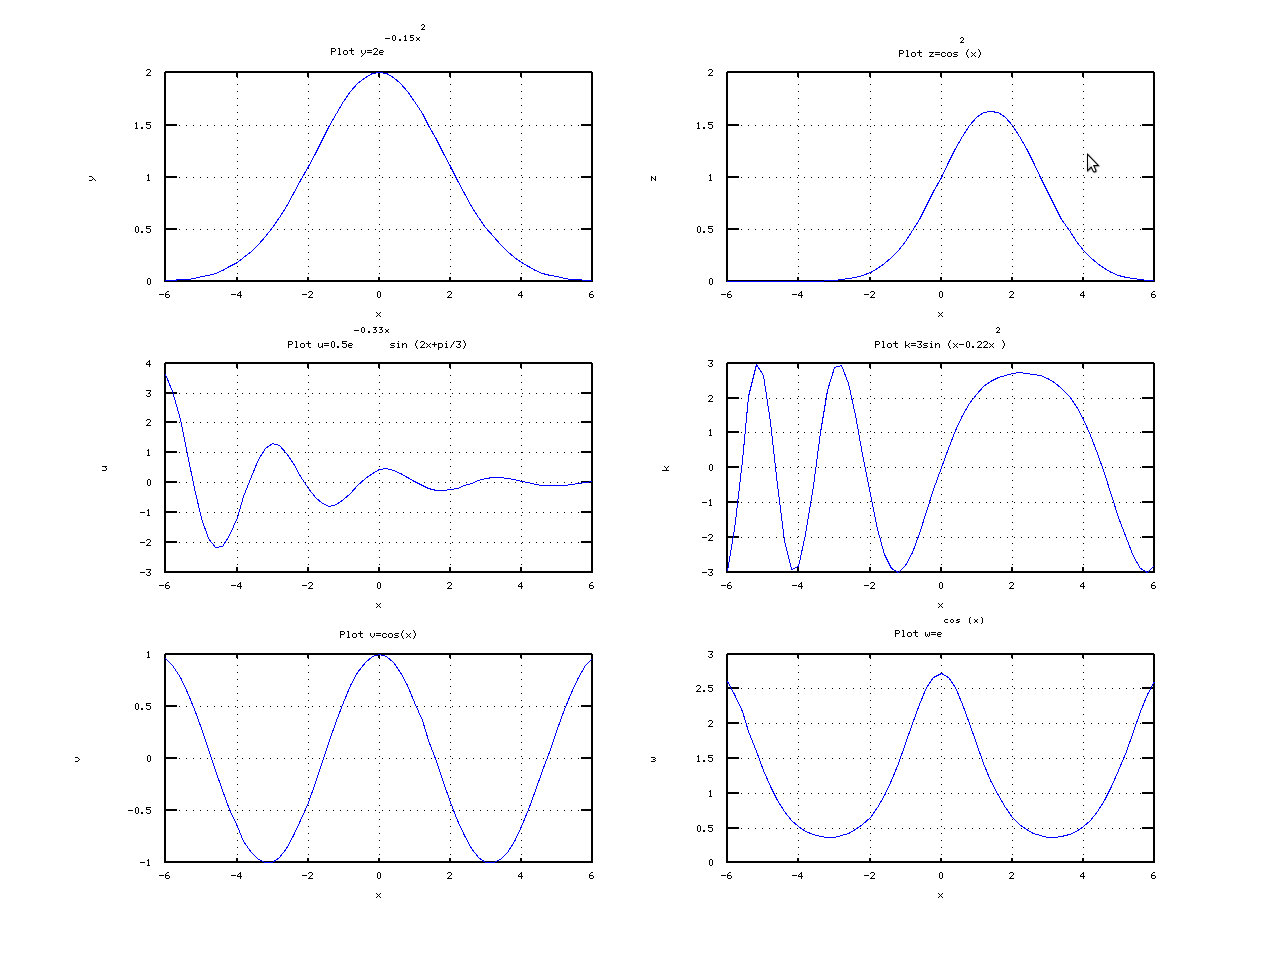
\includegraphics[width=8cm]{04_aer_octave_fig1.png}}
\caption{Графики графики нескольких функций в одном окне}
\label{pic:1}
\end{figure}

\begin{figure}[ht]
\centering{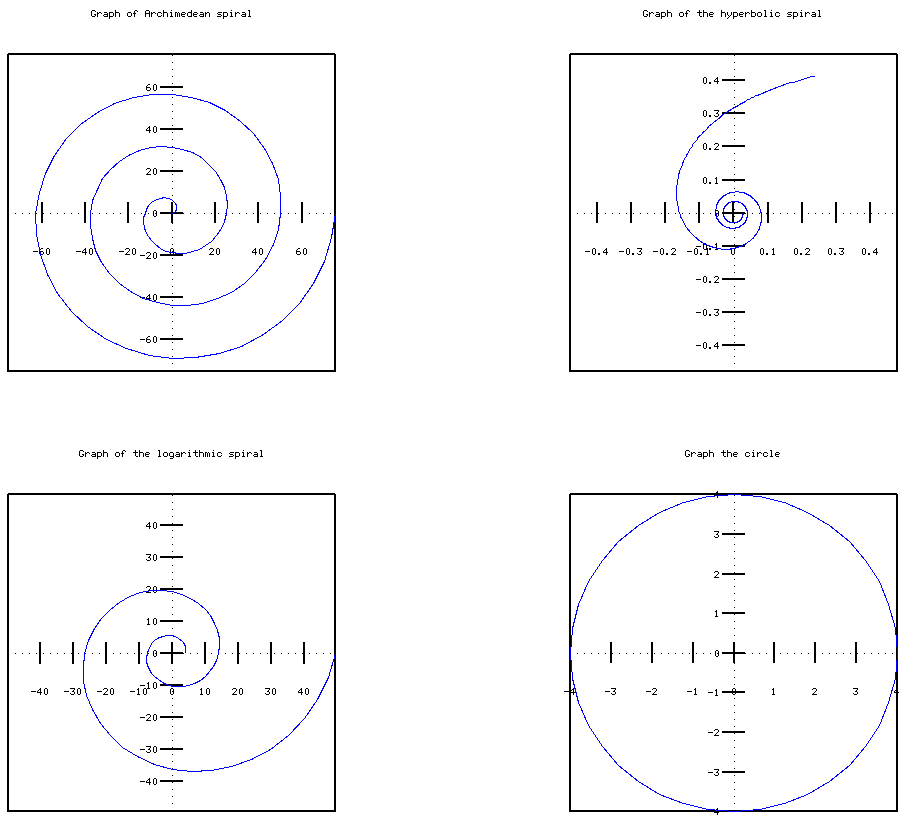
\includegraphics[width=8cm]{04_aer_octave_fig2.png}}
\caption{ Графики архимедовой, гиперболической и логарифмической спирали, окружности в полярных координатах}
\label{pic:2}
\end{figure}

\begin{figure}[ht]
\centering{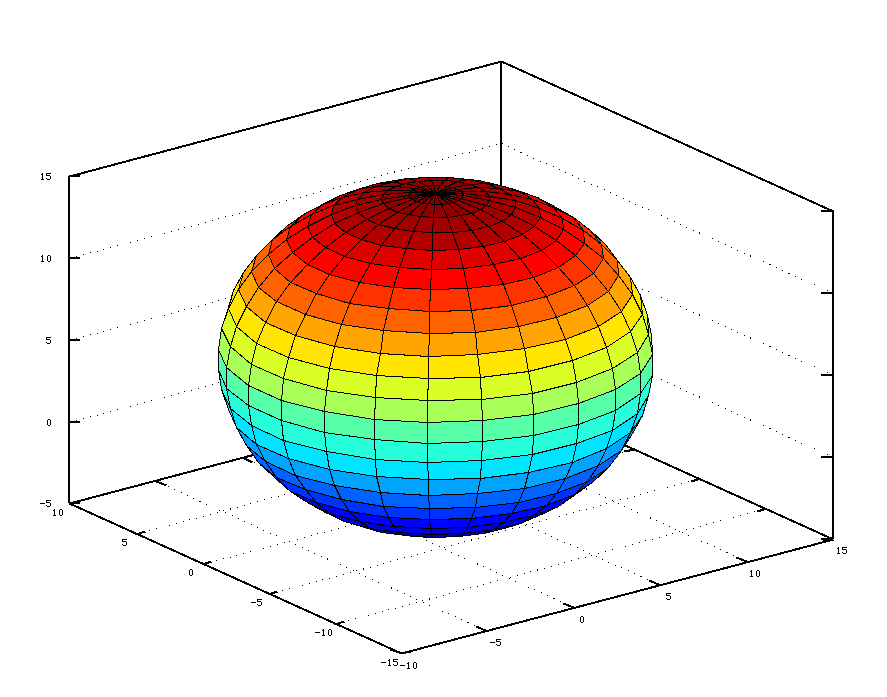
\includegraphics[width=8cm]{04_aer_octave_fig3.png}}
\caption{График сферы}
\label{pic:3}
\end{figure}

Octave содержит большое количество функций, предназначенных для решения задач линейной алгебры, наиболее используемые из них: \verb!det(M)! --- вычисляет определитель квадратной матрицы \verb!M!, \verb!norm(M[,p])! --- возвращает различные виды норм матрицы \verb!M! в зависимости от \verb!p!, \verb!inv(M)! --- возвращает матрицу обратную к \verb!M!, \verb!eig(M)! --- возвращает вектор собственных значений матрицы \verb!M!, \verb!rref(M)! --- осуществляет приведение матрицы \verb!M! к треугольной форме, используя метод исключения Гаусса, \verb!lu(M)!, \verb!qr (M)! --- выполняют LU и QR-разложение соответственно. 

Мощная графическая и математическая база  Octave позволяет решать задачи векторной алгебры и аналитической геометрии.

Octave содержит функции для численного и аналитического решения нелинейных уравнений и систем, а также для интегрирования и дифференцирования.

Оптимизационные задачи чаще всего решают с помощью проприетарного табличного процессора MS Excel. Однако, наиболее мощные и гибкие функции для решения подобных задач присутствуют именно в Octave. Так, для  решения линейных и нелинейных оптимизационных задач с ограничениями можно использовать функцию sqp, а для решения любых задач линейного программирования есть функция glpk. Сложные оптимизационные задачи в Octave решают с помощью пакета пакета расширений Minimization для GNU Octave (\url{http://octave.sourceforge.net/optim/overview.html}).

В инженерной практике часто приходится сталкиваться с решением обыкновенных дифференциальных уравнений и систем. В Octave существует достаточно много функций для решения обыкновенных уравнений и систем (в том числе и жёстких). Наиболее часто используемые среди них:
\begin{itemize}
\item \verb!ode23!, \verb!ode45! --- функции решений обыкновенных нежёстких дифференциальных уравнений (или систем) методом Рунге-Кутта 2-3-го и 4-5-го порядка точности соответсвенно,
\item \verb!ode5r!, \verb!ode2r! --- функции решений обыкновенных жёстких дифференциальных уравнений (или систем).
\end{itemize}

\begin{figure}[ht]
\centering{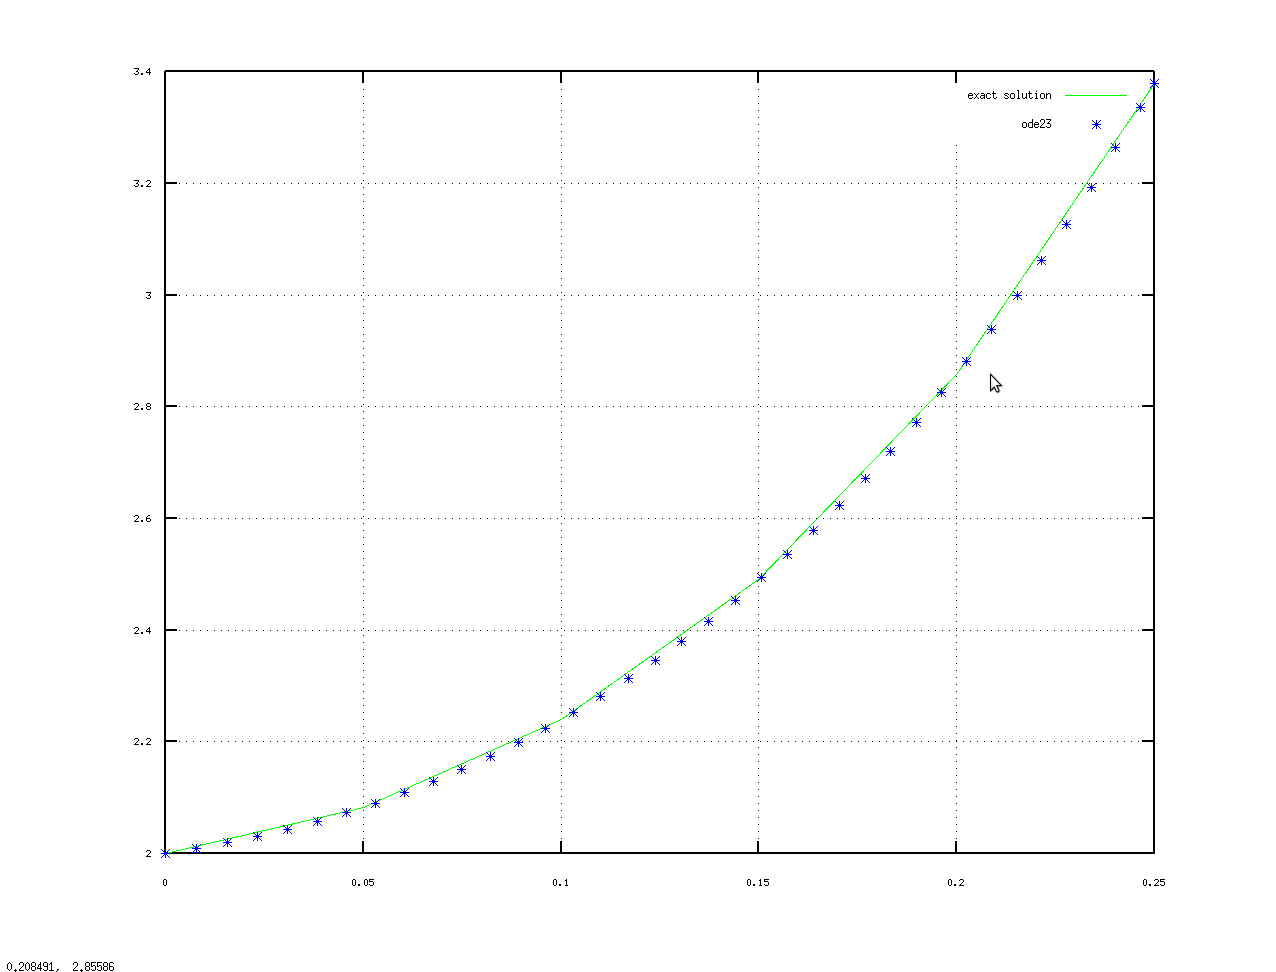
\includegraphics[width=8cm]{04_aer_octave_fig4.png}}
\caption{Графики точного решения (--) дифференциального уравнений и решения (*), найденного с помощью ode23}
\label{pic:4}
\end{figure}

Множество функций для решения дифференциальных уравнений находится в пакете расширений odepkg. Краткое описание функций этого пакета на английском языке с некоторыми примерами приведено на странице \url{http://octave.sourceforge.net/odepkg/overview.html}.

Также в Octave можно решать практически любые задачи обработки эксперимента. Для подбора параметров аналитической зависимости методом наименьших квадратов используются следующие функции: \verb!polyfit! --- подбор коэффициентов полинома k-й степени; \verb!sqp! --- функция поиска минимума.

Сплайн-интерполяция в Octave реализуется с помощью функции \verb!interp1!, которая позволяет  построить кубический и линейный сплайн.

C помощью Octave можно решать и много других задач. Авторами подготовлен учебник по использованию пакете GNU Octave, который будет опубликован в ближайшее время в Москве, в серии учебников ALT Linux, а также небольшим тиражом в Донецком национальном техническом университете. Рабочие материалы книги можно увидеть на сайте \url{http://gnu-octave.narod2.ru}.

Рассмотренные возможности Octave позволяют авторам рекомендовать пакет как инструмент для решения математических задач в курсах <<Высшая математика>>, <<Математический анализ>>, <<Линейная алгебра>>, <<Аналитическая геометрия>>, а также во многих специальных курсах, в которых приходится решать задачи вычислительной математики.
\end{document}






\newpage

\makeatletter
\let\enddocument\@lvee@enddoc
\let\input\@lvee@input
\makeatother

\eof


